%\documentclass[smaller, dvipsnames, handout]{beamer}
\def\bmode{0} % Mode 0 for presentation, mode 1 for a handout with notes, mode 2 fo% r handout without notes
\if 0\bmode
\documentclass[usenames,dvipsnames,smaller]{beamer}
\else \if 1\bmode
\immediate\write18{pdflatex -jobname=\jobname-Handout-Notes\space\jobname}
\documentclass[usenames,dvipsnames,smaller,handout]{beamer}
\usepackage{handoutWithNotes}
\pgfpagesuselayout{2 on 1 with notes}[letterpaper, landscape, border shrink=4mm]
\else \if 2\bmode
\immediate\write18{pdflatex -jobname=\jobname-Handout\space\jobname}
\documentclass[usenames,dvipsnames,smaller,handout]{beamer}
\fi
\fi
\fi

%\setbeamertemplate{section in head/foot}{}
%\setbeamertemplate{section in head/foot shaded}{\textcolor{white}{\insertsectionhead}}
%%%%%%%%%%%%%%%%%%%%%%%%%%%%%%%%%%%%%%%%%%%%%%%%%%%%%%%%%%%%%%%%%%%%%%%%%%%%%%%%%%%%%%%%%%%%%
\newcommand{\coursetitle}{CEE 697M: Probabilistic Machine Learning}
\newcommand{\longlecturetitle}{M4 Nonparametric Methods:\\ L4c: Support Vector Machines}
\newcommand{\shortlecturetitle}{L4c: SVM}
\newcommand{\instructor}{Jimi Oke}
\newcommand{\lecturedate}{Wed, Apr 26, 2023}
%%%%%%%%%%%%%%%%%%%%%%%%%%%%%%%%%%%%%%%%%%%%%%%%%%%%%%%%%%%%%%%%%%%%%%%%%%%%%%%%%%%%%%%%%%%%%

 
 
% \usepackage[T1]{fontenc} 
% \usepackage{lmodern} 
%\usepackage{etex}
 %\newcommand{\num}{6{} }

% \usetheme[
%   outer/progressbar=foot,
%   outer/numbering=fraction,
%   block=fill,
%   inner/subsectionpage=progressbar
% ]{metropolis}
\usetheme{Madrid}
\useoutertheme[subsection=false]{miniframes} % Alternatively: miniframes, infolines, split
\useinnertheme{circles}
% %\useoutertheme{Frankfurt}
% \usecolortheme{beaver}
% %\useoutertheme{crane}
% %\useoutertheme{metropolis}
\usepackage[backend=biber,style=authoryear,maxcitenames=2,maxbibnames=99,safeinputenc,url=false, eprint=false]{biblatex}
%\addbibresource{bib/references.bib}
% \AtEveryCitekey{\iffootnote{{\tiny}\tiny}{\tiny}}

% %\usepackage{pgfpages}
% %\setbeameroption{hide notes} % Only slides
% %\setbeameroption{show only notes} % Only notes
% %\setbeameroption{hide notes} % Only notes
% %\setbeameroption{show notes on second screen=right} % Both

% % \usepackage[sfdefault]{Fira Sans}

% % \setsansfont[BoldFont={Fira Sans}]{Fira Sans Light}
% % \setmonofont{Fira Mono}

% %\usepackage{fira}
% %\setsansfont{Fira}
% %\setmonofont{Fira Mono}
% % To give a presentation with the Skim reader (http://skim-app.sourceforge.net) on OSX so
% % that you see the notes on your laptop and the slides on the projector, do the following:
% % 
% % 1. Generate just the presentation (hide notes) and save to slides.pdf
% % 2. Generate onlt the notes (show only nodes) and save to notes.pdf
% % 3. With Skim open both slides.pdf and notes.pdf
% % 4. Click on slides.pdf to bring it to front.
% % 5. In Skim, under "View -> Presentation Option -> Synhcronized Noted Document"
% %    select notes.pdf.
% % 6. Now as you move around in slides.pdf the notes.pdf file will follow you.
% % 7. Arrange windows so that notes.pdf is in full screen mode on your laptop
% %    and slides.pdf is in presentation mode on the projector.

% % Give a slight yellow tint to the notes page
% \setbeamertemplate{note page}{\pagecolor{yellow!5}\insertnote}\usepackage{palatino}

% %\usetheme{metropolis}
% %\usecolortheme{beaver}
 \usepackage{tipa}
% \usepackage{enumerate}
\definecolor{darkcandyapplered}{HTML}{A40000}
\definecolor{lightcandyapplered}{HTML}{e74c3c}

% %\setbeamercolor{title}{fg=darkcandyapplered}

% \definecolor{UBCblue}{rgb}{0.04706, 0.13725, 0.26667} % UBC Blue (primary)
% \definecolor{UBCgrey}{rgb}{0.3686, 0.5255, 0.6235} % UBC Grey (secondary)

% % \setbeamercolor{palette primary}{bg=darkcandyapplered,fg=white}
% % \setbeamercolor{palette secondary}{bg=darkcandyapplered,fg=white}
% % \setbeamercolor{palette tertiary}{bg=darkcandyapplered,fg=white}
% % \setbeamercolor{palette quaternary}{bg=darkcandyapplered,fg=white}
% % \setbeamercolor{structure}{fg=darkcandyapplered} % itemize, enumerate, etc
% % \setbeamercolor{section in toc}{fg=darkcandyapplered} % TOC sections
% % \setbeamercolor{frametitle}{fg=darkcandyapplered,bg=white} % TOC sections
% % \setbeamercolor{title in head/foot}{bg=white,fg=white} % TOC sections
% % \setbeamercolor{button}{fg=darkcandyapplered} % TOC sections

% % % Override palette coloring with secondary
% % \setbeamercolor{subsection in head/foot}{bg=lightcandyapplered,fg=white}

%\usecolortheme{crane}
% \makeatletter
% \setbeamertemplate{headline}{%
%   \begin{beamercolorbox}[colsep=1.5pt]{upper separation line head}
%   \end{beamercolorbox}
%   \begin{beamercolorbox}{section in head/foot}
%     \vskip1pt\insertsectionnavigationhorizontal{\paperwidth}{}{}\vskip1pt
%   \end{beamercolorbox}%
%   \ifbeamer@theme@subsection%
%     \begin{beamercolorbox}[colsep=1.5pt]{middle separation line head}
%     \end{beamercolorbox}
%     \begin{beamercolorbox}[ht=2.5ex,dp=1.125ex,%
%       leftskip=.3cm,rightskip=.3cm plus1fil]{subsection in head/foot}
%       \usebeamerfont{subsection in head/foot}\insertsubsectionhead
%     \end{beamercolorbox}%
%   \fi%
%   \begin{beamercolorbox}[colsep=1.5pt]{lower separation line head}
%   \end{beamercolorbox}
% }
% \makeatother

% Reduce size of frame box
\setbeamertemplate{frametitle}{%
    \nointerlineskip%
    \begin{beamercolorbox}[wd=\paperwidth,ht=2.0ex,dp=0.6ex]{frametitle}
        \hspace*{1ex}\insertframetitle%
    \end{beamercolorbox}%
}


%\setbeamercolor{frametitle}{bg=darkcandyapplered!80!black!90!white}
%\setbeamertemplate{frametitle}{\bf\insertframetitle}

%\setbeamercolor{footnote mark}{fg=darkcandyapplered}
%\setbeamercolor{footnote}{fg=darkcandyapplered!70}
%\Raggedbottom
%\setbeamerfont{page number in head/foot}{size=\tiny}
%\usepackage[tracking]{microtype}


% %\usepackage[sc,osf]{mathpazo}   % With old-style figures and real smallcaps.
% %\linespread{1.025}              % Palatino leads a little more leading

% % Euler for math and numbers
% %\usepackage[euler-digits,small]{eulervm}
% %\AtBeginDocument{\renewcommand{\hbar}{\hslash}}
\usepackage{graphicx}
\usepackage{multirow}
\usepackage{booktabs}
\usepackage{graphbox}
\usepackage{animate}
\usepackage{media9}
\usepackage{adjustbox}

% %\mode<presentation> { \setbeamercovered{transparent} }

\setbeamertemplate{navigation symbols}{}
\makeatletter
\def\beamerorig@set@color{%
  \pdfliteral{\current@color}%
  \aftergroup\reset@color
}
\def\beamerorig@reset@color{\pdfliteral{\current@color}}
\makeatother


% %=== GRAPHICS PATH ===========
\graphicspath{{./m5-images/}}
% % Marginpar width
% %Marginpar width
% %\setlength{\marginparsep}{.02in}


% %% Captions
% % \usepackage{caption}
% % \captionsetup{
% %   labelsep=quad,
% %   justification=raggedright,
% %   labelfont=sc
% % }

% \setbeamerfont{caption}{size=\footnotesize}
% \setbeamercolor{caption name}{fg=darkcandyapplered}

% %AMS-TeX packages

\usepackage{amssymb}
\usepackage{amsmath}
\usepackage{amsthm}
\usepackage{mathtools} 
\usepackage{bm}
\DeclareMathOperator*{\argmax}{arg\,max}
\DeclareMathOperator*{\argmin}{arg\,min}
% \usepackage{color}

% %https://tex.stackexchange.com/a/31370/2269
\usepackage{cancel}
\renewcommand{\CancelColor}{\color{red}} %change cancel color to red
\makeatletter
\let\my@cancelto\cancelto %copy over the original cancelto command
\newcommand<>{\cancelto}[2]{\alt#3{\my@cancelto{#1}{#2}}{\mathrlap{#2}\phantom{\my@cancelto{#1}{#2}}}}
% redefine the cancelto command, using \phantom to assure that the
% result doesn't wiggle up and down with and without the arrow
\makeatother


% % \usepackage{comment}
\usepackage{enumerate}
\usepackage{hyperref}
% \usepackage{minitoc,array}
% \definecolor{slblue}{rgb}{0,.3,.62}
\hypersetup{
    colorlinks,%
    citecolor=blue,%
    filecolor=blue,%
    linkcolor=blue,
    urlcolor=blue
}

% \usepackage{epstopdf}
% \epstopdfDeclareGraphicsRule{.gif}{png}{.png}{convert gif:#1 png:\OutputFile}
% \AppendGraphicsExtensions{.gif}

% %\usepackage{listings}

% %%% TIKZ
\usepackage{forest}
\usepackage{tikz}
\usepackage{tikz-3dplot}
\usepackage{pgfplots}
\usepackage{pgfplotstable}
% \usepackage{pgfgantt}
\usepackage{neuralnetwork}

\usetikzlibrary{fit,arrows,arrows.meta,shapes,positioning,shapes.geometric}
\usetikzlibrary{decorations.markings}
\usetikzlibrary{shadows,automata}
\usetikzlibrary{patterns}
\usetikzlibrary{trees,mindmap,backgrounds}
%\usetikzlibrary{circuits.ee.IEC}
\usetikzlibrary{decorations.text}
% % For Sagnac Picture
% \usetikzlibrary{%
%     decorations.pathreplacing,%
%     decorations.pathmorphing%
% }
% \tikzset{no shadows/.style={general shadow/.style=}}
% %
% %\usepackage{paralist}

\tikzset{
  font=\Large\sffamily\bfseries,
  red arrow/.style={
    midway,red,sloped,fill, minimum height=3cm, single arrow, single arrow head extend=.5cm, single arrow head indent=.25cm,xscale=0.3,yscale=0.15,
    allow upside down
  },
  black arrow/.style 2 args={-stealth, shorten >=#1, shorten <=#2},
  black arrow/.default={1mm}{1mm},
  tree box/.style={draw, rounded corners, inner sep=1em},
  node box/.style={white, draw=black, text=black, rectangle, rounded corners},
}

% %%% FORMAT PYTHON CODE
% %\usepackage{listings}
% % Default fixed font does not support bold face
% \DeclareFixedFont{\ttb}{T1}{txtt}{bx}{n}{8} % for bold
% \DeclareFixedFont{\ttm}{T1}{txtt}{m}{n}{8}  % for normal

% % Custom colors
% \definecolor{deepblue}{rgb}{0,0,0.5}
% \definecolor{deepred}{rgb}{0.6,0,0}
% \definecolor{deepgreen}{rgb}{0,0.5,0}

% %\usepackage{animate}

% % Python style for highlighting
% % \newcommand\pythonstyle{\lstset{
% % language=Python,
% % basicstyle=\footnotesize\ttm,
% % otherkeywords={self},             % Add keywords here
% % keywordstyle=\footnotesize\ttb\color{deepblue},
% % emph={MyClass,__init__},          % Custom highlighting
% % emphstyle=\footnotesize\ttb\color{deepred},    % Custom highlighting style
% % stringstyle=\color{deepgreen},
% % frame=tb,                         % Any extra options here
%     % showstringspaces=false            % 
% % }}

% % % Python environment
% % \lstnewenvironment{python}[1][]
% % {
% % \pythonstyle
% % \lstset{#1}
% % }
% % {}

% % % Python for external files
% % \newcommand\pythonexternal[2][]{{
% % \pythonstyle
% % \lstinputlisting[#1]{#2}}}

% % Python for inline
% % 
% % \newcommand\pythoninline[1]{{\pythonstyle\lstinline!#1!}}

% %\usepackage{algorithm2e}

\newcommand{\eps}{\epsilon}
\newcommand{\bX}{\mb X}
\newcommand{\by}{\mb y}
\newcommand{\bbe}{\bm\beta}
\newcommand{\beps}{\bm\epsilon}
\newcommand{\bY}{\mb Y}

\newcommand{\osn}{\oldstylenums}
\newcommand{\dg}{^{\circ}}
\newcommand{\lt}{\left}
\newcommand{\rt}{\right}
\newcommand{\pt}{\phantom}
\newcommand{\tf}{\therefore}
\newcommand{\?}{\stackrel{?}{=}}
\newcommand{\fr}{\frac}
\newcommand{\dfr}{\dfrac}
\newcommand{\ul}{\underline}
\newcommand{\tn}{\tabularnewline}
\newcommand{\nl}{\newline}
\newcommand\relph[1]{\mathrel{\phantom{#1}}}
\newcommand{\cm}{\checkmark}
\newcommand{\ol}{\overline}
\newcommand{\rd}{\color{red}}
\newcommand{\bl}{\color{blue}}
\newcommand{\pl}{\color{purple}}
\newcommand{\og}{\color{orange!90!black}}
\newcommand{\gr}{\color{green!40!black}}
\newcommand{\lbl}{\color{CornflowerBlue}}
\newcommand{\dca}{\color{darkcandyapplered}}
\newcommand{\nin}{\noindent}
\newcommand*\circled[1]{\tikz[baseline=(char.base)]{
            \node[shape=circle,draw,thick,inner sep=1pt] (char) {\small #1};}}

\newcommand{\bc}{\begin{compactenum}[\quad--]}
\newcommand{\ec}{\end{compactenum}}

\newcommand{\p}{\partial}
\newcommand{\pd}[2]{\frac{\partial{#1}}{\partial{#2}}}
\newcommand{\dpd}[2]{\dfrac{\partial{#1}}{\partial{#2}}}
\newcommand{\pdd}[2]{\frac{\partial^2{#1}}{\partial{#2}^2}}
\newcommand{\pde}[3]{\frac{\partial^2{#1}}{\partial{#2}\partial{#3}}}
\newcommand{\nmfr}[3]{\Phi\left(\frac{{#1} - {#2}}{#3}\right)}
\newcommand{\Err}{\text{Err}}
\newcommand{\err}{\text{err}}

\DeclarePairedDelimiter\ceil{\lceil}{\rceil}
\DeclarePairedDelimiter\floor{\lfloor}{\rfloor}

%%%% GREEK LETTER SHORTCUTS %%%%%
\newcommand{\la}{\lambda}
\renewcommand{\th}{\theta}
\newcommand{\al}{\alpha}
\newcommand{\G}{\Gamma}
\newcommand{\si}{\sigma}
\newcommand{\Si}{\Sigma}


\pgfmathdeclarefunction{poiss}{1}{%
  \pgfmathparse{(#1^x)*exp(-#1)/(x!)}%
  }

\pgfmathdeclarefunction{gauss}{2}{%
  \pgfmathparse{1/(#2*sqrt(2*pi))*exp(-((x-#1)^2)/(2*#2^2))}%
}

\pgfmathdeclarefunction{expo}{2}{%
  \pgfmathparse{#1*exp(-#1*#2)}%
}

\pgfmathdeclarefunction{expocdf}{2}{%
  \pgfmathparse{1 -exp(-#1*#2)}%
}

\newcommand{\mb}{\mathbb}
\newcommand{\mc}{\mathcal}
\newcommand{\tr}{^{\top}}
\newcommand{\empt}[2]{$#1^{( #2 )}$}
\newcommand{\pe}{\pause}
% \usepackage{pst-plot}

% \usepackage{pstricks-add}
% \usepackage{auto-pst-pdf}   

% \psset{unit = 3}

% \def\target(#1,#2){%
%  {\psset{fillstyle = solid}
%   \rput(#1,#2){%
%     \pscircle[fillcolor = white](0.7,0.7){0.7}
%     \pscircle[fillcolor = blue!60](0.7,0.7){0.5}
%     \pscircle[fillcolor = white](0.7,0.7){0.3}
%     \pscircle[fillcolor = red!80](0.7,0.7){0.1}}}}
% \def\dots[#1](#2,#3){%
%     \psRandom[
%       dotsize = 2pt,
%       randomPoints = 25
%     ](!#2 #1 0.04 sub sub #3 #1 0.04 sub sub)%
%      (!#2 #1 0.04 sub add #3 #1 0.04 sub add)%
%      {\pscircle[linestyle = none](#2,#3){#1}}}


%%%%%%%%%%%%%%%%%%%%%%%%%%%%%%%%%%%%%%%%%%%%%%%%%%%
%%%%%%%%%%%%%%%%%%%%%%%%%%%%%%%%%%%%%%%%%%%%%%%%%%%
\title[\shortlecturetitle]{ {\normalsize \coursetitle}
  \\ \longlecturetitle}
\date[\lecturedate]{\footnotesize \lecturedate}
\author{{\bf \instructor}}
\institute[UMass Amherst]{
%\titlegraphic{\hfill
  \begin{tikzpicture}[baseline=(current bounding box.center)]
    \node[anchor=base] at (-7,0) (its) {\includegraphics[scale=.3]{UMassEngineering_vert}} ;
  \end{tikzpicture}
  % \hfill\includegraphics[height=1.5cm]{logo}
}

%https://tex.stackexchange.com/questions/55806/mindmap-tikzpicture-in-beamer-reveal-step-by-step
  \tikzset{
    invisible/.style={opacity=0},
    visible on/.style={alt={#1{}{invisible}}},
    alt/.code args={<#1>#2#3}{%
      \alt<#1>{\pgfkeysalso{#2}}{\pgfkeysalso{#3}} % \pgfkeysalso doesn't change the path
    },
  }


% https://tex.stackexchange.com/questions/446468/labels-with-arrows-for-an-equation
% https://tex.stackexchange.com/a/402466/121799
\newcommand{\tikzmark}[3][]{
\ifmmode
\tikz[remember picture,baseline=(#2.base)] \node [inner sep=0pt,#1](#2) {$#3$};
\else
\tikz[remember picture,baseline=(#2.base)] \node [inner sep=0pt,#1](#2) {#3};
\fi
}

% \lstset{language=matlab,
%                 basicstyle=\scriptsize\ttfamily,
%                 keywordstyle=\color{blue}\ttfamily,
%                 stringstyle=\color{blue}\ttfamily,
%                 commentstyle=\color{gray}\ttfamily,
%                 morecomment=[l][\color{gray}]{\#}
%               }


%%% Local Variables:
%%% mode: latex
%%% TeX-master: t
%%% End:

              
\begin{document}
\maketitle
\begin{frame}
  \frametitle{Outline}
  \tableofcontents
\end{frame}



 
  
\section{Introduction}
\begin{frame}
  \frametitle{Key concepts}
  \pause
  \begin{itemize}[<+->]
  \item The\textit{\bl maximal margin classifier} partitions perfectly separable observations using a \textit{\og separating hyperplane}.
  \item \textit{\rd Support vector classifiers} extend the \textit{\bl maximal margin classifier} by allowing for observations to overlap the linear decision boundary.
  \item  \textit{\pl Support vector machines (SVM)} generalize the \textit{\rd support vector classifier} by using kernels to allow for nonlinear decision boundaries.
\end{itemize}
\pause
\begin{alertblock}{Extensions}
  \begin{itemize}[<+->]
  \item SVM can be modified for regression problems (SVM regression)
  \item Can also be used for multiclass problems
  \item Can be regularized for improved performance
  \item Outputs can be converted to probabilities (Platt scaling)
  \end{itemize}
\end{alertblock}
\end{frame}

 
% \begin{frame}
%   \frametitle{Variable importance in random forests}

%   %   \begin{figure}[h!]
%   %     \centering
%   %     \visible<6->{\includegraphics[width=.75\textwidth, trim={4.5cm 8cm 4cm 4.4cm}, clip]{ESL15-5}}
%   %     \caption{}
%   % \end{figure}


% \end{frame}

\begin{frame}
  \frametitle{Hyperplane}
  \pause
  
  \begin{block}{Definition}
    A hyperplane is an affine\footnote{Generalization of Euclidean} subspace of dimension $D-1$ in a $D$-dimensional affine space. \pause
    It partitions a space in two.
  \end{block}
  \pause
  
  \begin{minipage}[b]{.45\linewidth}
  \begin{figure}[h!]
  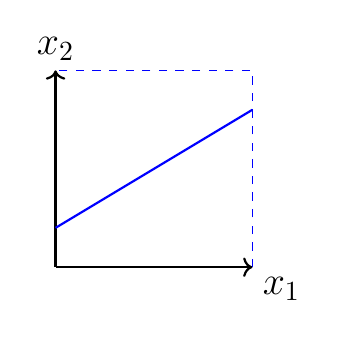
\begin{tikzpicture}[scale=2.5]
    \visible<3->{\draw[thick,->] (0,0) -- (1,0) node[anchor=north west]{$x_1$};}
    \visible<4->{\draw[thick,->] (0,0) -- (0,1) node[anchor=south]{$x_2$};}
    \visible<5->{\draw[thin,dashed,blue] (1,0) -- (1,1) -- (0,1);}
    \visible<6->{\draw[blue,thick] (0,0.2) -- (1,.8);}
  \end{tikzpicture}
  \pause
  \visible<7->{\caption{Separating hyperplane in 2D}}
\end{figure}
\end{minipage}\hfill
\begin{minipage}[b]{.45\linewidth}
\begin{figure}[h!]
  \tdplotsetmaincoords{70}{110}
\begin{tikzpicture}[scale=2.5,tdplot_main_coords]
  \visible<8->{\draw[thick,->] (0,0,0) -- (1,0,0) node[anchor=north east]{$x_1$};}
  \visible<8->{\draw[thick,->] (0,0,0) -- (0,0,1) node[anchor=south]{$x_3$};}
    \def\x{.5}
    % \draw[thin] (0,0,0) -- ({1.2*\x},{sqrt(3)*1.2*\x},0) node[below] {$y=\sqrt{3}x$};
    \visible<9->{\draw[thin,dashed,blue] (0,0,1) -- (1,0,1) -- (1,1,1) -- (0,1,1) -- cycle;}
    \visible<9->{\draw[thin,dashed,blue] (0,0,0) -- (1,0,0) -- (1,1,0) -- (0,1,0) -- cycle;}
    \visible<10->{    \filldraw[
        draw=blue,thick,%
        fill=blue!20,%
    ]          (1,0,0.5)
            -- (1,1,0.5)
            -- (0,1,0.5)
            -- (0,0,0.5)
            -- cycle;}
    \visible<9->{\draw[thin,dashed,blue] (1,0,1) -- (1,0,0);}
    \visible<9->{\draw[thin,dashed,blue] (1,1,1) -- (1,1,0);}
    \visible<9->{\draw[thin,dashed,blue] (0,1,1) -- (0,1,0);}
    \visible<8->{\draw[thick,->] (0,0,0) -- (0,1,0) node[anchor=north west]{$x_2$};}
\end{tikzpicture}
\visible<11->{\caption{Separating hyperplane in 3D}}
\end{figure}
\end{minipage}
\end{frame}

% \begin{frame}
%   \frametitle{Hyperplane}

%   \begin{block}{Definition}
%     A hyperplane is a flat affine\footnote{Generalization of Euclidean} subspace of dimension $p-1$ in a $p$-dimensional affine space.
%   \end{block}
  
%   \tdplotsetmaincoords{70}{110}
% \begin{tikzpicture}[scale=2.5,tdplot_main_coords]
%     \draw[thick,->] (0,0,0) -- (1,0,0) node[anchor=north east]{$x$};
%     \def\x{.5}
%     \draw[thin] (0,0,0) -- ({1.2*\x},{sqrt(3)*1.2*\x},0) node[below] {$y=\sqrt{3}x$};
%     \filldraw[
%         draw=blue,%
%         fill=blue!20,%
%     ]          (0,0,0)
%             -- (\x,{sqrt(3)*\x},0)
%             -- (\x,{sqrt(3)*\x},1)
%             -- (0,0,1)
%             -- cycle;
%     \draw[thick,->] (0,0,0) -- (0,1,0) node[anchor=north west]{$y$};
%     \draw[thick,->] (0,0,0) -- (0,0,1) node[anchor=south]{$z$};
% \end{tikzpicture}
% \end{frame}

% \begin{frame}
%   \frametitle{Hyperplane (cont.)}\pause
%   \begin{itemize}[<+->]
%   \item In two dimensions, we see that a hyperplane is simply a straight line:\pause
%     \begin{equation}
%       \label{eq:1}
%        w_0 +  w_1 x_1 +  w_2 x_2 = 0
%     \end{equation}\pause
%     All points/vectors $(x_{i1},x_{i2})$ satisfying Eq.\ \eqref{eq:1} lie on the hyperplane. \pause

%       \begin{figure}[h!]
%         \begin{tikzpicture}[scale=2.5]
%           \visible<5->{\draw[thick,->] (0,0) -- (1,0) node[anchor=north west]{$x_1$};
%           \draw[thick,->] (0,0) -- (0,1) node[anchor=south]{$x_2$};
%           \draw[thin,dashed,blue] (1,0) -- (1,1) -- (0,1);}
%           \visible<6->{\draw[blue,thick] (0,0.2) -- (1,.8);}
%           \visible<7->{\draw[orange!80!black] (0.4,0.44) node[circle,fill,inner sep=2pt,label=below:$a$](a){};}
%           \visible<8->{\draw[orange!80!black] (1,0.8) node[circle,fill,inner sep=2pt,label=below right:$b$](b){};}
%         \end{tikzpicture}       
%         \visible<+->{\caption{Points on a hyperplane in 2D: $ w_0 = 0.2,  w_1 = 0.6,  w_2 = -1.0$}}
%       \end{figure}

%     \pause
%   \item In {\rd three} dimensions, a hyperplane is a \textit{plane}:\pause
%     \begin{equation}
%       \rd       w_0 +  w_1 x_1 +  w_2 x_2 +  w_3 x_3 = 0
%     \end{equation}
%   \end{itemize}
% \end{frame}

\begin{frame}
  \frametitle{Hyperplane --- generalization}
  \pause
  \visible<2->{In $D$ dimensions, a hyperplane is then given by:}
  \visible<3->{\begin{equation}
     w_0 +  w_1 x_1 +  w_2 x_2 + \cdots +  w_D x_D = 0
  \end{equation}}
  \vspace{-2ex}
  \begin{itemize} 
    \visible<6->{ \item $D+1$ parameters are required to define  hyperplane}
    \visible<7->{  \item Relative to a hyperplane, points can be located in three distinct regions:}
  \end{itemize}
    \pause
    \begin{eqnarray}
      \visible<8->{ w_0 +  w_1 x_1 +  w_2 x_2 + \cdots +  w_D x_D &=& 0 \quad\og \text{(on hyperplane itself)} \\}
      \visible<10->{ w_0 +  w_1 x_1 +  w_2 x_2 + \cdots +  w_D x_D &<& 0 \quad \pl \text{(\textit{one} side of hyperplane)} \\}
      \visible<12->{ w_0 +  w_1 x_1 +  w_2 x_2 + \cdots +  w_D x_D &>& 0 \quad \gr \text{(\textit{other} side of hyperplane)}}
    \end{eqnarray}
    \vspace{-1ex}
    \begin{figure}[h!]
      \tdplotsetmaincoords{70}{110}
      \begin{tikzpicture}[scale=1,tdplot_main_coords]
        \visible<4->{\draw[thin,dashed,blue] (0,-2,1) -- (2,-2,1) -- (2,4,1) -- (0,4,1) -- cycle;
          \draw[thin,dashed,blue] (0,-2,0) -- (2,-2,0) -- (2,4,0) -- (0,4,0) -- cycle;
          \draw[thin,dashed,blue] (2,-2,1) -- (2,-2,0);
          \draw[thin,dashed,blue] (2,4,1) -- (2,4,0);
          \draw[thin,dashed,blue] (0,4,1) -- (0,4,0);
          \draw[thin,dashed,blue] (0,-2,1) -- (0,-2,0);
          \draw[thick,->,gray,dashed] (0,0,0) -- (2,0,0) node[anchor=east]{$x_1$};
          \draw[thick,->,gray,dashed] (0,0,0) -- (0,4,0) node[anchor=west]{$x_2$};
          \draw[thick,->,gray,dashed] (0,0,0) -- (0,0,1) node[anchor=east]{$x_3$};}
        \visible<5->{\filldraw[draw=blue,thick,fill=blue!20]
          (2,-2,1)
          -- (0,-2,1)
          -- (0,4,0)
          -- (2,4,0)
          -- cycle;}        
        \visible<9->{\draw[orange!80!black] (1,-2,1) node[circle,fill,inner sep=2pt,label=left:$a$](a){};}
        \visible<11->{\draw[purple] (1,-2,0) node[circle,fill,inner sep=2pt,label=left:$b$](b){};}
        \visible<13->{\draw[green!50!black] (0.5,3.5,1) node[circle,fill,inner sep=2pt,label=above right:$c$](c){};}              
      \end{tikzpicture}
      \visible<14->{\caption{Separating hyperplane in three dimensions}}
    \end{figure}
\end{frame}

% \begin{frame}
%   \frametitle{Separating hyperplane}\pause
%   \begin{block}{Definition}
%     A $D-1$ separating hyperplane is one that perfectly partitions $D$-dimensional datapoints by their binary class labels.
%   \end{block}
%   \pause
%   \begin{figure}[h!]
%     \centering
%     \visible<3->{\includegraphics[width=.45\textwidth, trim={0cm 0cm 11cm 0cm}, clip]{9-2}}
%     \vspace{-1ex}
%     \visible<4->{\caption{Three separating hyperplanes in a 2D setting}}
%   \end{figure}
% \end{frame}

\begin{frame}
  \frametitle{Separating hyperplanes}
  \pause
  Supposing a $\widetilde{y}\in\{-1,+1\}$ class coding for a $D$-dimensional dataset, then a separating hyperplane satisfies the following conditions: \pause
  \begin{equation}
    \label{eq:2}
    \begin{cases}
       w_0 +  w_1 x_1 +  w_2 x_2 + \cdots +  w_D x_D > 0, & \pause \widetilde{y}_n = +1 \\\pause
       w_0 +  w_1 x_1 +  w_2 x_2 + \cdots +  w_D x_D < 0, & \pause \widetilde{y}_n = -1 
    \end{cases}
  \end{equation}
  \pause
  
  \begin{minipage}[]{.58\linewidth}
    Let\pause
    \begin{equation}
      f(\bm x) =  w_0 +  w_1 x_1 +  w_2 x_2 + \cdots +  w_D x_D
    \end{equation}
    \pause
    Multiplying
    $f(\bm x)$ by $\widetilde{y}_n$, \pause we see that Eq.\ \eqref{eq:2} is equivalent to: 
  \pause
  \begin{equation}\bl
    \label{eq:3}
    \boxed{ \widetilde{y}_n \cdot f(\bm x_n) > 0}
  \end{equation}
  \pause


\end{minipage}
\hfill
\begin{minipage}[]{.35\linewidth}
    \begin{figure}[h!]
    \centering
    \visible<10->{\includegraphics[width=.9\textwidth, trim={11cm 0cm 0cm 0cm}, clip]{9-2}}
    \vspace{-1ex}
    \visible<11->{\caption{Selected separating hyperplane used as decision rule for classification}}
  \end{figure}
\end{minipage}
\end{frame}


\begin{frame}
  \frametitle{Separating hyperplane (summary)}
  \pause
  \begin{itemize}[<+->]
  \item Using a $\widetilde{y}\in \{-1,+1\}$ class coding, we assign a point $x^*$ by:\pause
    \begin{equation}
      \widetilde{y}_{x^*} = \text{sign}\{f(\bm x^*)\}
    \end{equation}
    \pause
    where
    \begin{equation}
      f(\bm x^*) =        w_0 +  w_1 x^*_1 +  w_2 x^*_2 + \cdots +  w_D x^*_D
    \end{equation}
  \begin{itemize}[<+->]
  \item If   $f(\bm x^*)$ is negative, the $n$th observation is assigned to Class $-1$.
  \item If   $f(\bm x^*)$ is positive, the $n$th observation is assigned to Class $+1$.
%  \item Equivalently, 
\end{itemize}
  \item The magnitude of $f(\bm x^*)$ indicates the certainty of the assignment
    \begin{itemize}[<+->]
    \item If $f(\bm x^*)$ is large, then $\bm x^*$ is further away from the hyperplane and thus there is less uncertainty about its class prediction
    \end{itemize}
  \item Using a separating hyperplane as a decision rule is equivalent to estimating a \textit{linear} decision boundary.
  \end{itemize}
  
\end{frame}


\section{Maximal margin classifier}
\begin{frame}
  \frametitle{Distance between a point and hyperplane}
  \pause
  % Recall the dot product between two vectors $\bm x_1$ and $\bm x_2$:
  % \begin{equation}
  %   \bm x_1 \cdot \bm x_2 = \pause ||\bm x_1|| ||\bm x_2|| \cos \theta
  % \end{equation}
  % \pause
  % Now, for any two points $x_1$ and $x_2$ on a hyperplane $L$:
  % \begin{equation}
  %   ( w_1,  w_2, \ldots,  w_D)\tr (x_1 - x_2) = \pause = \bm w\tr (x_1 -x_2) = \pause 0
  % \end{equation}
  % \pause
  % Using the dot product definition,
  The unit normal vector to the surface of a hyperplane $L$ is given by:\pause
  \begin{equation}
    \bl \bm w^* = \pause \fr{\bm w}{||\bm w||}
  \end{equation}
  \pause
  where we define the vector $\bm w$ as
  \begin{equation}
    \bm w =  ( w_1,  w_2, \ldots,  w_D)
  \end{equation}
  \pause
  For any point $\bm x_n$ in $L$:
  \begin{equation}
     w_0 + \bm w\tr \bm x_n = 0 \pause    \quad\implies\quad {\rd \bm w\tr \bm x_n =} \pause {\rd - w_0}
  \end{equation}
  \pause
  Finally, the {\gr\bf signed distance} of a point $\bm x_{n}$ to the hyperplane $L$ is given by:\pause
  \begin{eqnarray}
    \begin{split}
      \gr \bm w^{*T}(\bm x - \bm x_n)  &= \pause {\bl \fr{1}{||\bm w||}} \bm w\tr (\bm x - \bm x_n) = \pause
      \fr{1}{||\bm w||}\lt(\bm w\tr \bm x - \bm w\tr \bm x_n\rt)\\ \pause
      &= \pause \fr{1}{||\bm w||}\lt( \bm w\tr \bm x - {\rd (- w_0)}\rt)
      = \pause  \fr{1}{||\bm w||}\lt(\bm w\tr \bm x +  w_0\rt) = \pause \gr \fr{1}{||f'(\bm x)||}f(\bm x)
    \end{split}
  \end{eqnarray}
\end{frame}

\begin{frame}
  \frametitle{Distance between a point and a hyperplane (illustrated)}
  \pause

   \begin{figure}[h!]
    \centering
     \visible<2->{\includegraphics[width=.75\textwidth, trim={0cm 9cm 0cm 5cm}, clip]{ESL4-15}}
    \vspace{-1ex}
  \end{figure}
  
  \pause
  The perpendicular distance between a point $\bm x_{n}$ and a hyperplane is given by: \pause

  \begin{equation}
  ||(x- x_0)||\cos\theta =  \pause        \fr{\bm w\tr (\bm x - \bm x_n)}{||\bm w||} \pause =  \bm w^{*T}(\bm x - \bm x_n)  
  \end{equation}
  
%   \begin{center}
%   \begin{tikzpicture}[scale=.7]
% \begin{axis}[width=5in,clip=false,axis equal image,
%     axis lines=middle,
%     xmin=-7,xmax=7,
%     ymin=-7,ymax=7,
%     xlabel=$x$,ylabel=$y$,
%     restrict y to domain=-7:7,
%     enlargelimits={abs=0.5cm},
%     axis line style={latex-latex},
%     ticklabel style={font=\tiny,fill=white},
%     xtick={\empty},ytick={\empty},
%     xlabel style={at={(ticklabel* cs:1)},anchor=north west},
%     ylabel style={at={(ticklabel* cs:1)},anchor=south west}
% ]

% \addplot[latex-latex,samples=2,domain=-7:7,blue, thick] {(2/3)*x - 1} 
%     coordinate [pos=0] (s) 
%     coordinate (e)
%     node[anchor=south east,pos=0.9,font=\footnotesize]{$y=\dfrac{2}{3}x - 1$};

% \draw[dashed,
%     decoration={brace,raise=5pt,amplitude=5pt},
%     postaction={draw,solid,decorate}] 
%     ($(s)!0.5!(e)$) coordinate (m) --($($(s)!0.5!(e)$)!0.8!90:(e)$)
%      node[circle,inner sep=2pt,fill=blue,label={[blue,font=\footnotesize]45:$P$}] (p){}
%     ($($(m)!0.5!(p)$)!10pt!90:(p)$) node[anchor=east] {$d$};

% \draw[fill=white] ($(m)!3mm!(e)$) coordinate (U) 
%      -- ($(U)!3mm!90:(e)$) -- ($(m)!3mm!(p)$) -- (m) -- cycle;

% \end{axis}
% \end{tikzpicture}
% \end{center}

\end{frame}

\begin{frame}
  \frametitle{Margin of a separating hyperplane}
  \pause
     The \textbf{margin} of a separating hyperplane is the smallest [perpendicular] distance from the hyperplane to any of the observations. \pe
    \begin{equation}
      M = \min_{n=1}^{N}\bm w^{*\top}(\bm x - \bm x_{n}) \pe =
      \min_{n=1}^{N}[\widetilde{y}_{n} (w_{0} + \bm w\tr \bm x_{n})]
    \end{equation}

  \pause
  \begin{minipage}[b]{.45\linewidth}
    \begin{itemize}[<+->]
    \item The datapoints defining the margin are called \textbf{support vectors}
    \item In the figure on the right the support vectors for hyperplane $B$ are shown
    \item Can you identify the support vectors for $A$? How many are there?
    \end{itemize}
  \end{minipage}\hfill\pause
  \begin{minipage}[b]{.46\linewidth}
  \begin{figure}[h!]
    \centering
    % \visible<6->{\includegraphics[width=.4\textwidth, trim={0cm 1cm 0cm 0cm}, clip]{9-3}}
    \visible<6->{\includegraphics[width=.95\textwidth]{mmh}}
    \vspace{-1ex}
    \visible<7->{\caption{Margins of two separating hyperplanes}}
  \end{figure}
\end{minipage}

\end{frame}

\begin{frame}
  \frametitle{Optimal separating hyperplane}
  \pause
  \begin{itemize}[<+->]
  \item A perfectly separable dataset has an infinite number of separating hyperplanes
  \item We can use \textbf{maximal margin} criterion to select the optimal separating hyperplane:
    \begin{itemize}[<+->]
    \item Define the margin as $M$
    \item Find/choose the separating hyperplane for which $M$ is the largest
    \end{itemize}
  \item Thus the optimal separating hyperplane is also called the \textbf{maximal margin hyperplane}
  \end{itemize}
  \pause
  \begin{figure}[h!]
    \centering
    % \visible<6->{\includegraphics[width=.4\textwidth, trim={0cm 1cm 0cm 0cm}, clip]{9-3}}
    \visible<7->{\includegraphics[width=.4\textwidth]{mmh}}
    \vspace{-1ex}
    \caption{\visible<8->{Margins of two separating hyperplanes.}
      \visible<9->{Which of the two is optimal? Why?}
    \visible<10->{{\gr Hyperplane $A$ is the maximal margin hyperplane}}}
  \end{figure}  
\end{frame}

\begin{frame}
  \frametitle{Finding the maximal margin classifier}
  \pause
  Using the optimal separating hyperplane as a decision rule produces the \textbf{maximal margin classifier}.
  \pause
  
  Formally, this is the solution to the optimization problem:\pause
  \alert{\begin{equation}
  \max_{\bm w, M}  M   
\end{equation}\pause
\quad\quad  subject to \pause
  \begin{eqnarray}\label{eq:mmcc1}
    \sum_{d=1}^D w_d^2 &=& ||\bm w||\pause = 1 \\ \label{eq:mmcc2} \pause
    \widetilde{y}_n( w_0 + \bm w\tr \bm x_n) &\ge& M \quad \pause \forall n = 1, \ldots, N
  \end{eqnarray}
  }
  \pause
  Recall that the distance between a point $x$ and a hyperplane is
  $ \fr{1}{||\bm w||}\lt(\bm w\tr \bm x_{n} +  w_0\rt) $.
  \pause
  Thus, \alert{Constraint \eqref{eq:mmcc1}} ensures that we can obtain the distance between a point $\bm x_n$ and the hyperplane by \pause
  \begin{equation}
    d_n = \widetilde{y}_n( w_0 + \bm w\tr \bm x_n)
  \end{equation}
  \pause
  And \alert{Constraint \eqref{eq:mmcc2}} assures that the distance between all training observations and the classifier will be no less than $M$.
\end{frame}


\section{Support vector classifier}


\begin{frame}
  \frametitle{Overlapping of classes}
  \pause
  \begin{itemize}[<+->]
  \item When observations do not overlap, then separating hyperplanes exist and a maximal margin classifier can be found
   \item If observations overlap,  there is no solution to the maximal margin classifier 
  \item We must relax the optimization problem to allow for minimal observations to fall on the wrong side of the margin  
   \item We do this using \textit{slack variables} (producing a \textbf{soft margin})
  \item The resulting optimization problem results in the \textbf{support vector classifier}
  \end{itemize}

    \begin{figure}[h!]
      \centering
      \visible<6->{\includegraphics[width=.3\textwidth, trim={0cm 0cm 44cm 0cm}, clip]{svmsvc}} \quad\quad
      \visible<7->{\includegraphics[width=.3\textwidth, trim={44cm 0cm 0cm 0cm}, clip]{svmsvc}}            
      \caption{\tiny (Left) \textbf{Maximal margin classifier:} only possible if data are perfectly separable. (Right) \textbf{Support vector
        classifier:} relaxes the margin and allows observations to fall on the wrong side of margin (M) and hyperplane
        (H).  {\tiny Source:
        \url{https://www.surveypractice.org/article/2715-using-support-vector-machines-for-survey-research} }}
  \end{figure}
  
\end{frame}

% \begin{frame}
%   \frametitle{Maximal margin vs.\ support vector classifiers}
% \pause
%   \begin{figure}[h!]
%       \centering
%       \visible<2->{\includegraphics[width=.45\textwidth, trim={0cm 0cm 44cm 0cm}, clip]{svmsvc}}
%       \visible<3->{\includegraphics[width=.45\textwidth, trim={44cm 0cm 0cm 0cm}, clip]{svmsvc}}            
%       \caption{(Left) \textbf{Maximal margin classifier:} only possible if data are perfectly separable. (Right) \textbf{Support vector
%         classifier:} relaxes the margin and allows observations to fall on the wrong side of margin (M) and hyperplane
%         (H).  {\tiny Source:
%         \url{https://www.surveypractice.org/article/2715-using-support-vector-machines-for-survey-research} }}
%   \end{figure}
% \end{frame}

% \begin{frame}
%   \frametitle{Support vector classifier}\pause
%   \begin{itemize}[<+->]
%   \item Allows for classification of overlapping observations using a soft margin
%   \item More robust to changes in training data
%   \end{itemize}
%   \pause

%   \begin{block}{Non-robustness of maximal margin classifier}
%     \begin{figure}[h!]
%     \centering
%     \visible<4->{\includegraphics[width=.35\textwidth, trim={0cm 0cm 11cm 0cm}, clip]{9-5}}\quad
%     \visible<6->{\includegraphics[width=.35\textwidth, trim={11cm 0cm 0cm 0cm}, clip]{9-5}}
%      % \visible<6->{\includegraphics[width=.4\textwidth]{mmh}}
%     \vspace{-1ex}
%     \visible<5->{\caption{
%         Addition of one observation drastically alters optimal hyperplane.}}
%   \end{figure}    
%   \end{block}

% \end{frame}

\begin{frame}
  \frametitle{Finding the support vector classifier}
  \pause
  The support vector classifier is the solution to:\pause
  \alert{  \begin{equation}
  \max_{ w_0,\bm w, \xi}  M   
\end{equation}\pause
\quad\quad  subject to\pause
  \begin{eqnarray}\label{eq:7}
    \sum_{d=1}^D w_d^2 &=& ||\bm w|| = 1 \\ \pause \label{eq:8}
    \widetilde{y}_n( w_0 + \bm w\tr \bm x_n) &\ge& M (1 - \xi_n) \quad \forall n = 1, \ldots, N \\\pause
    \xi_n &\ge& 0 \\\pause
    \sum_{n=1}^{N} \xi_n &\le& B
  \end{eqnarray}}
\pause
  \begin{itemize}[<+->]
  \item $\xi_n$ are \textbf{slack variables} allowing the $n$th observation to be on the wrong side (overlap)
  \item $B$ is a nonnegative tuning parameter (``\textbf{budget''}), which moderates the size of the allowable overlap.
      \item If $\xi_n = 0$ for all $i$, then the problem solves the \textbf{maximal margin classifier}

 \end{itemize}

\end{frame}


\begin{frame}
  \frametitle{Slack variables in SVC}
  \pause
   Slack variable $\xi_n$ behavior for $n$th observation:\pause
   \begin{equation}
     \xi_n\pause
     \begin{cases}
       = 0, &  \pause \text{correct side of margin}\\\pause
       > 0, &  \pause \text{wrong side of margin}\\\pause
       > 1, &  \pause \text{wrong side of hyperplane (overlapping)}
     \end{cases}
   \end{equation}
   \pause
  \begin{itemize}[<+->]\rd 
  \item Observations directly on the margin ($\xi_n=0$) or on the wrong side of the margin ($\xi_1 > 0$) are the \textbf{support vectors}
  % \item The larger the cost parameter $C$, the wider the margin
  \end{itemize}
  \medskip
  \pause
  
  \begin{minipage}[t]{.3\linewidth}
    \centering
    \visible<6->{\includegraphics[width=.9\textwidth, trim={8.5cm 0cm 0cm 1cm}, clip]{9-6}}
    \pause
    
    {\footnotesize SVC for a small dataset}
  \end{minipage}\hfill\pause
  \begin{minipage}[t]{.68\linewidth}
    %   \visible<8->{\begin{figure}[h!]
    %     \centering
    %     % \visible<6->{\includegraphics[width=.4\textwidth]{mmh}}
    % \vspace{-1ex}
    % \caption{
    \begin{itemize}\footnotesize
    \item Class {\color{violet}Violet}:\pause
      \begin{itemize}\scriptsize
      \item  Point {\color{violet}  11} is on   wrong side of   hyperplane ($\xi_{11}>1$) \pause
    \item Pt.\ {\color{violet} 1} is on   wrong side of   margin ($\xi_{1}>0$)\pause
    \item Pt.\  {\color{violet} 2} is on   margin ($\xi_{2}=0$)\pause
      \end{itemize}
    \item Class {\lbl Sky Blue}:\pause
      \begin{itemize} \scriptsize
      \item Pt.\ {\lbl 12} is on   wrong side of   hyperplane\pause
      \item Pt.\ {\lbl 8} is on   wrong side of   margin\pause
      \item Pt.\  {\lbl 7} and {\lbl 9} are on   margin\pause
      \end{itemize}
    \item The \textbf{support vectors/points} are: \pause {\color{violet} 1}, {\color{violet} 2}, {\color{violet} 11},
    \pause {\lbl 7},  {\lbl 8}, {\lbl 9} and {\lbl
        12}.
    \end{itemize}

    %}
  %\end{figure}
\end{minipage}
\end{frame}


\begin{frame}
  \frametitle{Budget parameter and the bias-variance tradeoff}
  \pause
  \begin{itemize}[<+->]
  \item $B$ determines the width of the margin (tolerance of overlap)
  \item Typically, $B$ is chosen via $k$-fold cross-validation
  \item As $B$ becomes larger, the percentage of training observations that are support vectors increases (i.e.\ more observations are on the wrong side of margin or hyperplane)
  \item Large $B$  increases bias (more misclassifications)
but reduces  variance (greater stability)
    
  \end{itemize}
  \pause
  \begin{figure}[h!]
    \centering
    \visible<7->{\includegraphics[width=.22\textwidth, trim={0cm 9.5cm 10cm 0cm}, clip,align=c]{9-7}}
    \visible<8->{\includegraphics[width=.22\textwidth, trim={10cm 9.5cm 0cm 0cm}, clip,align=c]{9-7}}
    \visible<9->{\includegraphics[width=.22\textwidth, trim={0cm 0cm 10cm 10.1cm}, clip,align=c]{9-7}}
    \visible<10->{\includegraphics[width=.22\textwidth, trim={10cm 0cm 0cm 10.1cm}, clip,align=c]{9-7}}         
    \visible<6->{\caption{Support vector classifier: $B$ decreasing from Left to Right.}}
  \end{figure}
\end{frame}







\section{Optimization for SVC}


% \begin{frame}
%   \frametitle{Optimization problem I (OP1)}
%   \pause
%   The support vector classifier is the solution to :\pause
%   \begin{eqnarray}\label{eq:8}
%     \begin{split}
%       &       \max_{ w_0,\bm w, \xi}  M   \\  \pause
%       \text{subject to}\pause \quad  \sum_{d=1}^D w_d^2 &= ||\bm w|| = 1 \\ \pause 
%       \widetilde{y}_n( w_0 + \bm w\tr \bm x_n) &\ge M (1 - \xi_n) \quad \forall n = 1, \ldots, N \\\pause
%       \sum_{n=1}^{N} \xi_n &\le B \\\pause
%       \xi_n &\ge 0 
%     \end{split}
%   \end{eqnarray}
%   \pause
%   \begin{itemize}[<+->]
%   \item $\xi_n$ are slack variables allowing for overlap
%   \item $B$ (``budget'') moderates the size of the allowable overlap
%   \end{itemize}

% \end{frame}


\begin{frame}
  \frametitle{Reformulating \texttt{[OP1]}}
  \pause

  Recall that the \textit{signed} distance between a point $\bm x_n$ and a separating hyperplane $f(\bm x) =  w_0 + \bm w\tr x$ is given by:
  \begin{equation}
    \fr{1}{||\bm w||} ( w_0 + \bm w\tr  \bm x_n)
  \end{equation}
  Since $\widetilde{y}_n = \{-1, 1\}$, then the absolute distance is given by:\pause
  \begin{equation}
    \widetilde{y}_n\times \fr{1}{||\bm w||} ( w_0 + \bm w\tr  \bm x_n) 
  \end{equation}
  \pause
 
  \pause

  In OP1, constraining $\gr ||\bm w|| = 1$ allowed us to write the boundary constraint as:
  \begin{equation}
    \widetilde{y}_n\times \fr{1}{\gr||\bm w||} ( w_0 + \bm w\tr  \bm x_n) = \pause
    \widetilde{y}_n\times \fr{1}{\gr 1} ( w_0 + \bm w\tr  \bm x_n) \pause  \ge M (1 - \xi_n)
  \end{equation}
  \pause
  If instead we do not constrain $||\bm w||$, then the constraint can be written as:\pause
  \begin{equation}
    \widetilde{y}_n( w_0 + \bm w\tr  \bm x_n) \ge M||\bm w|| (1 - \xi_n)
  \end{equation}

\end{frame}


\begin{frame}
  \frametitle{Reformulating \texttt{[OP1]} (cont.)}
  \pause
  Now, let us set
  \begin{equation}
    M = \fr{1}{||\bm w||} \pause \quad \implies \quad \pause ||\bm w|| = \fr1M
  \end{equation}
  \pause
  Two implications follow:\pause
  \begin{itemize}[<+->]
  \item \textit{Maximizing} $M$ (the margin) is equivalent to \textit{minimizing} $||\bm w||$\\ \pause
  \item The boundary constraint becomes:\pause
    \begin{equation}
        \widetilde{y}_n( w_0 + \bm w\tr  \bm x_n) \ge M||\bm w|| (1 - \xi_n) = \pause M \cdot \fr 1M  (1 - \xi_n) = \pause  1 - \xi_n 
    \end{equation}
  \end{itemize}
  Given these, we can formulate a new optimization problem \texttt{OP2} to solve for the support vector classifier.
\end{frame}
\begin{frame}
  \frametitle{Optimization problem 2 \texttt{[OP2]}}
  \pause
  We can write the optimization problem for a support vector classifier as:\pause
  \begin{eqnarray}\label{eq:8}
    \begin{split}
      &       \min_{ w_0,\bm w, \xi}  \fr12|| \bm w ||^2  \\  \pause
      \text{subject to:} \pause \quad     \widetilde{y}_n( w_0 + \bm w\tr \bm x_n) &\ge 1 - \xi_n \quad \forall n = 1, \ldots, N \\\pause
      \sum_{n=1}^{N} \xi_n &\le B \\\pause
      \xi_n &\ge 0 
    \end{split}
  \end{eqnarray}
  \pause
  \begin{itemize}[<+->]
  \item     For computational convenience, we minimize $\fr12||\bm w||^2$ (a quadratic programming problem)
  \end{itemize}
\end{frame}

\begin{frame}
  \frametitle{Optimization problem 3 \texttt{[OP3]}}
  \pause
  The budget constraint can be included in the objective (penalty method) to obtain:
  \begin{eqnarray}\label{eq:8}
    \begin{split}
        \min_{ w_0,\bm w, \xi}  \lt( \fr12|| \bm w ||^2   +  C\sum_{n=1}^{N} \xi_n \rt) &\\  \pause
      \text{subject to}\pause \quad     \widetilde{y}_n( w_0 + \bm w\tr \bm x_n) &\ge 1 - \xi_n \quad \forall n  \\\pause
      \xi_n &\ge 0 
    \end{split}
  \end{eqnarray}
  \pause
  \begin{itemize}[<+->]
  \item In this form, we can see that $C\sum_{n=1}^{N} \xi_n$ serves as an overlap penalty
  \item We can now refer to $C$ as a ``cost'' parameter here
  \item As $C \to \infty$, \pause $\xi_n \to 0$
  \item Thus, a small $C$ allows for more overlap (larger margin), while a large $C$ leads to less overlap (smaller margin)
  \end{itemize}
\end{frame}

\begin{frame}
  \frametitle{Method of Lagrange multipliers}\pause
  Using the method of Lagrange multipliers we can write the Lagrangian form of the problem \texttt{[OP3]} and minimize that instead. \pause

  \medskip

  This is done by:
  \begin{itemize}[<+->]
  \item Rewriting each inequality constraint in the form $g(x)\ge 0$
  \item Augmenting the objective function by subtracting $\la g(x)$, where $\la$ is the Lagrange multiplier
  \item Solving the respective differential equations by setting the gradient of the Lagrangian $\mathcal{L}$ to 0 (w.r.t.\ each of the unknowns)
  \end{itemize}
  % \begin{eqnarray}
  %   \begin{split}
  %     \min_{ w_0,\bm w,\xi} L_D &= \fr12|| \bm w ||^2   +  C\sum_{n=1}^{N} \xi_n
  %     - \sum_{n=1}^{N}\alpha_n\lt[ \widetilde{y}_n( w_0 + \bm w\tr \bm x_n) -  1 - \xi_n  \rt] - \sum_{n=1}^{N}\mu_n\xi_n
  %   \end{split}
  % \end{eqnarray}
\end{frame}

\begin{frame}
  \frametitle{Method of Lagrange multipliers on \texttt{[OP3]}}\pause
  Given \texttt{[OP3]}:
  \begin{eqnarray}
    \begin{split}
        \min_{ w_0,\bm w, \xi}  \lt( \fr12|| \bm w ||^2   +  C\sum_{n=1}^{N} \xi_n \rt) &\\  \pause
      \text{subject to}\pause \quad     \widetilde{y}_n( w_0 + \bm w\tr \bm x_n) &\ge 1 - \xi_n \quad \forall n  \\\pause
      \xi_n &\ge 0 
    \end{split}
  \end{eqnarray}
  \pause
  we rewrite the constraints as:\pause
    \begin{eqnarray}
      %  \min_{ w_0,\bm w, \xi}  \lt( \fr12|| \bm w ||^2   +  C\sum_{n=1}^{N} \xi_n \rt) &&\\  \label{eq:10}\pause
      % \text{subject to:}\pause \quad   
      \label{eq:10} \widetilde{y}_n( w_0 + \bm w\tr \bm x_n) - ( 1 - \xi_n) &\ge& 0 \quad \forall n  \\ \label{eq:11}\pause
      \xi_n &\ge& 0 
    \end{eqnarray}
    \pause
    Let the Lagrange multiplier of Constraint \eqref{eq:10} be $\alpha_n$ and the Lagrange multiplier of Constraint \eqref{eq:11} be $\mu_n$.\pause
  \end{frame}


  \begin{frame}
  \frametitle{Primal Lagrangian problem}\pause
  Then we augment the objective to obtain the \textbf{primal Lagrangian} $\mc{L}_P$ as:
  \medskip
  \pause
  \begin{equation}
    \mathcal{L}_P = \fr12|| \bm w ||^2   +  C\sum_{n=1}^{N} \xi_n
    - \sum_{n=1}^{N}\alpha_n\lt[ \widetilde{y}_n( w_0 + \bm w\tr \bm x_n) -  1 + \xi_n  \rt] - \sum_{n=1}^{N}\mu_n\xi_n
  \end{equation}
  \pause
  To \textbf{minimize} $\mc{L}_P$, we find the gradient $\nabla\mathcal{L}_P$ (w.r.t.\ $ w_0$, $\bm w$ and $\xi$) and set to zero.\footnote{The subscript $P$ denotes that this is the primal problem, as there exists a dual problem that can be maximized.}
  \begin{eqnarray}
 \label{eq:13}   \nabla_{ w_0} &=&  -\sum_{n=1}^{N}\alpha_n\widetilde{y}_n = 0 \\\pause
 \label{eq:14}    \nabla_{\bm w} &=&  \bm w - \sum_{n=1}^{N}\alpha_n\widetilde{y}_n\bm x_n = 0 \\\pause
 \label{eq:15}    \nabla_{\xi} &=& C - \alpha_n - \mu_n = 0 
  \end{eqnarray}
\end{frame}

\begin{frame}
  \frametitle{Optimization problem 4 \texttt{[OP4]}: Dual Lagrangian}
  \pause
  Finally, we can substitute Constraints \eqref{eq:13}, \eqref{eq:14} and \eqref{eq:15} into $\mathcal{L}_D$ to obtain the dual Lagrangian
  objective function, which we \textbf{maximize}:\pause
  \begin{equation}\bl
   \max  \mathcal{L}_D = \pause \sum_{n=1}^{N}\alpha_n -
\fr12\sum_{n=1}^{N}\sum_{n'=1}^{N}\alpha_n\alpha_{n'}\widetilde{y}_ny_{n'}\bm x_n\tr \bm x_{n'}
  \end{equation}
  \pause
  subject to the \textbf{Karush-Kuhn-Tucker} (KKT) {\gr conditions}:\pause
  \begin{eqnarray}
    \gr    0 \le \alpha_n & \gr \le & \gr   C \\ \pause
    \gr    \sum_{n=1}^{N}\alpha_n\widetilde{y}_n &\gr =&\gr 0 \\ \pause
    \gr    \alpha_n\lt[ \widetilde{y}_n( w_0 + \bm w\tr \bm x_n) -  1 + \xi_n  \rt]  & \gr = & \gr 0 \\\pause
    \gr    \mu_n\xi_n & \og = & \gr 0 \\ \pause
    \gr    \widetilde{y}_n( w_0 + \bm w\tr \bm x_n) -  1 + \xi_n   & \gr \ge& \gr 0 
  \end{eqnarray}
  %\pause
  %Computationally, it is more convenient to solve the dual problem.
\end{frame}

\begin{frame}
  \frametitle{Support vector classifier solution form}\pause
  Recall constraint \eqref{eq:14} of the primal Lagrangian $\mc{L}_P$:\pause
  \begin{eqnarray}
    \bm w - \sum_{n=1}^{N}\alpha_n\widetilde{y}_n\bm x_n &=& 0 
  \end{eqnarray}
  This indicates that the coefficients of fitted classifier (hyperplane) are given by:\pause
  \begin{eqnarray}
        \hat{\bm w} &=& \sum_{n=1}^{N}\hat\alpha_n\widetilde{y}_n\bm x_n
  \end{eqnarray}
  \pause
  We observe that:\pause
  \begin{itemize}[<+->]
  \item When $\hat\alpha_n \ne 0$, then $\widetilde{y}_n( w_0 + \bm w\tr \bm x_n) -  1 + \xi_n = 0$
  \item Observations for which $\hat\alpha$ is nonzero are the \textbf{support vectors}
    \begin{itemize}
        \item  $\alpha_{n} < C$, \pause $\xi_n = 0$ (observation on margin)

        \item $\alpha_{n} = C$ : $\xi_{n} \le 1$: (obs.\ inside margin);\\
          \pe $\xi_{n} > 1$ (obs.\ lie on the wrong side of  hyperplane)         
\end{itemize}
    % \begin{eqnarray*}
    %   \mu_n\xi_n &=& 0 \\\pause
    %   \text{If $\xi_n \ne 0$, then } \mu_n &=& 0 \\\pause
    %   \therefore \hat\alpha_n &=& C -\mu_n = C - 0 = C
    % \end{eqnarray*}
  \end{itemize}
\end{frame}

\begin{frame}
  \frametitle{Estimating the intercept}
  \pe
  The decision boundary (hyperplane) of the fitted SVC is given by: \pe
  \begin{equation}
    f(\bm x; \hat w_{0}, \hat{\bm w}) = \hat w_{0} + {\gr \hat{\bm w}\tr} \bm x\pe
    = \hat w_{0} + {\gr \sum_{n=1}^{N}\hat\alpha_n\widetilde{y}_n\bm x_n\tr } \bm x
  \end{equation}
  \pe
  The intercept is estimated as:\pe
  \begin{equation}
    \hat w_{0} = \fr1{|\mc M|} \sum_{n\in \mc M} \lt(\widetilde{y}_{n} - \sum_{m\in \mc S} \hat\alpha_m\widetilde{y}_m\bm x_m\tr \bm x_{n}\rt)
  \end{equation}
  \pe
  where: \pe
  
  \begin{itemize}
  \item $\mc M$: set of points where $0 < \alpha_{n} < C$  (on margin)\pe
  \item $\mc S$: set of support vectors ($\alpha_{m} \ne 0$)
  \end{itemize}
\end{frame}



\section{Nonlinearity in SVC}




\begin{frame}
  \frametitle{Support vector classifier as inner product}

  \pause
  Recall the dual problem defining the support vector classifier:
  \pause
  \begin{equation}
    \mathcal{L}_D = \pause \sum_{n=1}^{N}\alpha_n - \fr12\sum_{n=1}^{N}\sum_{n'=1}^{N}\alpha_n\alpha_{n'}\widetilde{y}_ny_{n'}{\pl \bm x_n\tr \bm x_{n'}} \pause
    = \pause \sum_{n=1}^{N}\alpha_n - \fr12\sum_{n=1}^{N}\sum_{n'=1}^{N}\alpha_n\alpha_{n'}\widetilde{y}_ny_{n'}{\pl \langle \bm x_n, \bm x_{n'}\rangle }
  \end{equation}
  \pause
  We observed that the fitted coefficients of the classifier have the form:
  \pause
  \begin{equation}
    \hat{\bm w} = \sum_{n=1}^{N}\hat\alpha_n\widetilde{y}_n\bm x_n
  \end{equation}
  \pause
  Which means that the estimated classifier is given by:\pause
  \begin{eqnarray}
    \hat f(\bm x) &=&  \hat w_0 + \hat{\bm w}\tr \bm x \\ \pause
              &=&  \hat w_0 +  \lt(\sum_{n=1}^{N}\hat\alpha_n\widetilde{y}_n\bm x_n\rt)\tr \bm x \\\pause
                  &=& \hat w_0 + \sum_{n=1}^{N}\hat\alpha_n\widetilde{y}_n{\pl \bm x\tr \bm x_n} \pause
                      = \hat w_0 + \sum_{n=1}^{N}\hat\alpha_n\widetilde{y}_n {\pl \langle \bm x, \bm x_n\rangle}
  \end{eqnarray}
\end{frame}

\begin{frame}
  \frametitle{Nonlinear decision boundaries}
  \pause

  Suppose that even with a relaxed margin, a linear decision boundary performs poorly on a certain dataset?
  \pause
  \visible<+->{
  \begin{figure}[h!]
    \centering
    \includegraphics[width=.68\textwidth,trim={0 0.5cm 0 0},clip]{svc2}
    \caption{A case where a linear decision boundary performs poorly }
  \end{figure}}
  \pause
  \vspace{-1ex}
  How can we address this using a support vector classifier?
\end{frame}


\begin{frame}
  \frametitle{Expanding the feature space for nonlinear boundaries}
  \pause
  \begin{block}{}
  We can address nonlinearity by projecting the feature space into a larger dimensional space in which the boundary becomes linear.\pause
\end{block}
  \medskip
  
  Consider the hyperplane function (where $D=2$):
  \begin{equation}
    f(\bm x) =  w_0 + \bm w\tr \bm x =  w_0 +  w_1x_1 +  w_2x_2
  \end{equation}
  \pause
  We could perform a quadratic transformation:\pause
  \begin{equation}
    f^{*}(\bm x) =  w_0 + \bm {w}^{*\top}\phi(\bm x) 
  \end{equation}
  \pause
  where $\phi(\bm x) =
  \begin{pmatrix}
    x_1 \\[2mm] x_2\\[2mm]  x_1^2\\[2mm]   x_2^2
  \end{pmatrix}$
  \pause
   (feature extractor) and $\bm w'$ is  a $4 \times 1$ vector.

\end{frame}



\begin{frame}
  \frametitle{Generalizing the support vector classifier}
  \pause
  \begin{itemize}[<+->]
  \item  We can generalize the inner product in $\hat f(\bm x)$ as a basis expansion in $\bm x$ in order to obtain nonlinear decision boundaries.\pause

  \item   Let $\phi(\bm x)$ be a vector of functions/transformations of $x$.

  \item   Then we can substitute this into the Lagrangian:
    \pause
    \begin{equation}
    \mathcal{L}_D  
    = \pause \sum_{n=1}^{N}\alpha_n - \fr12\sum_{n=1}^{N}\sum_{n'=1}^{N}\alpha_n\alpha_{n'}\widetilde{y}_ny_{n'}{\pl \langle \phi(\bm x_n), \phi(\bm x_{n'})\rangle }
  \end{equation}
\item The resulting classifier then has the form:
  \begin{equation}
    \hat f(x) =  \hat{w}_0 + \sum_{n=1}^{N}\hat\alpha_n\widetilde{y}_n {\pl \langle \phi(\bm x), \phi(\bm x_n)\rangle}
  \end{equation}

\item This extension of the support vector classifier to allow for nonlinearity produces the \textbf{\pl support vector machine (SVM)}.
\end{itemize}
\end{frame}


\section{Support Vector Machines}
% \begin{frame}
%   \frametitle{The support vector machine (SVM)} \pause
%   The support vector machine obtained as the solution to: \pause
  
%     \alert{  \begin{equation}
%   \max_{ w_0,\bm w, \xi}  M   
% \end{equation}\pause
% \quad\quad  subject to\pause
%   \begin{eqnarray}\label{eq:7}
%     \sum_{d=1}^D w_d^2 &=& ||\bm w|| = 1 \\ \pause \label{eq:8}
%     \widetilde{y}_n( w_0 + \bm w\tr \bm x_n) &\ge& M (1 - \xi_n) \quad \forall n = 1, \ldots, N \\\pause
%     \xi_n &\ge& 0 \\\pause
%     \sum_{n=1}^{N} \xi_n &\le& C
%   \end{eqnarray}}
% \end{frame}

\begin{frame}
  \frametitle{The kernel trick}\pe
  More generally, we specify the basis expansion of the inner product of the inputs via Mercer \textbf{\gr kernel} functions:\pe
  % the kernel transformation to generalize the transformation of the inner product $\mc{K}(\bm x_n, x_{n'})$

  \begin{equation}\gr
    \mc{K}(\bm x, \bm x') =  \langle \phi(\bm x), \phi(\bm x')\rangle 
  \end{equation}
  \pe
  The {\bl linear kernel} is simply:\pe
  \begin{equation}\bl
    \mc{K}(\bm x, \bm x') =  \langle \bm x, \bm x'\rangle 
  \end{equation}\pe
  
  which produces a linear boundary ({\bl suport vector classifier}).
  \pause

  \medskip
  
  Other common inner-product kernel choices are:
  \begin{eqnarray}
    \pl \text{\bf Polynomial of degree $\bm d$:}\quad \pause  \mc{K}(\bm x, \bm x') &=& \pl (1 + \langle \bm x, \bm x'\rangle )^d \\ \label{eq:rbf} \pe
    \gr    \text{\bf Radial basis function (RBF):}\quad \pause  \mc{K}(\bm x, \bm x') &=& \gr \exp(-\gamma ||\bm x - \bm  x'||^2 ) \\ \pe
    \og \text{\bf Neural network (sigmoid):}\quad \pause  \mc{K}(\bm x, \bm x') &=& \og \tanh(1 + \kappa_1\langle \bm x, \bm x'\rangle + \kappa_2 ) 
  \end{eqnarray}
\end{frame}
\begin{frame}
  \frametitle{SVM general solution form}\pause
  The support vector machine is also the solution to the Lagrangian dual problem:\pause
  \begin{eqnarray}
    \begin{split}
      \max \mathcal{L}_D &= \sum_{n=1}^{N}\alpha_n - \fr12\sum_{n=1}^{N}\sum_{n'=1}^{N}\alpha_n\alpha_{n'}\widetilde{y}_ny_{n'}{\pl  \mc{K}(\bm x_n, \bm x_{n'})  }       
  \end{split}   
  \end{eqnarray}
  \pause
  where $\pl \mc{K}(\bm x_n,\bm x_{n'}) $ is a \textbf{Mercer kernel} specifying the inner product expansion in the feature space.\pause
  \medskip
 
   Therefore the {\bl SVM solution}  has the form:
  \begin{equation}\bl
    \hat f(\bm x) = \sum_{n=1}^{N} \hat\alpha_n \widetilde{y}_n  \mc{K}(\bm x_n, \bm x)  + \hat w_0
  \end{equation}
  \pause

  The beauty of the kernel transformation is that the inner products in $\mc{K}(\bm x_{n}, \bm x)$
  can be cheaply computed without explicitly specifying high-dimensional basis function expansions $\phi(\bm x)$.

\end{frame}



\begin{frame}
  \frametitle{More on the radial kernel}
  \pause
  The {\gr radial kernel transformation} has a localizing effect on the distance measurement. \pause

  \begin{itemize}[<+->]
  \item As defined in Eq.\ \eqref{eq:rbf}, it is a Gaussian function
  \item The localization effect increases with $\gamma$ (leading to a more flexible decision boundary)
  \end{itemize}

  \includegraphics<5->[width=.47\textwidth]{rbf1}\hfill
    \includegraphics<5->[width=.47\textwidth]{rbf2}
\end{frame}
\begin{frame}
  \frametitle{Example: polynomial kernel of degree 2}
  \pause
  Consider a case with two inputs $x_1$ and $x_2$.
  \pause
  We can write the degree-2 polynomial kernel as follows:
  \begin{eqnarray}\label{eq:2dkern}
    \begin{split}
    \mc{K}(\bm x, \bm x') &= (1 + \langle \bm x, \bm x' \rangle )^2  \pause
              = (1 + x_1x_1' + x_2x_2')^2 \\\pause
            &= 1 + 2x_1x_1' + 2x_2x_2' + (x_1x_1')^2 + (x_2x_2')^2 + 2x_1x_1'x_2x_2'
          \end{split}
  \end{eqnarray}
  \pause
  Explicitly, this is an inner product of basis functions $\phi(\bm x)$:\pause
  \begin{eqnarray}\label{eq:2dh}
    \begin{split}
    \mc{K}(\bm x, \bm x') &=\pause
              \begin{pmatrix}
                \\
                1 & x_1\sqrt 2 & x_2\sqrt 2 & x_1^2 & x_2^2 & x_1x_2\sqrt 2\\
                \\
              \end{pmatrix}\pause
                  \begin{pmatrix}
                1 \\[2mm] x_1'\sqrt 2 \\[2mm] x_2'\sqrt 2 \\[2mm] {x}_1'^{2} \\[2mm] {x}_2'^{2} \\[2mm] x_1' x_1'\sqrt 2
              \end{pmatrix} \\\pause
            &= \phi(\bm x)\tr \phi(\bm x') =  \left\langle \phi(\bm x), \phi(\bm x') \right\rangle
          \end{split}
  \end{eqnarray}
  \pause
  % In practice, it is not necessary to specify $\phi(\bm x)$
\end{frame}

\begin{frame}
  \frametitle{Example: SVM degree-2 polynomial (quadratic) kernel}
  \pause
  \visible<+->{
  \begin{figure}[h!]
    \centering
    \includegraphics[width=.68\textwidth,trim={0 0.5cm 0 0},clip]{svc3}
    \caption{A quadratic decision boundary produced on the earlier dataset using an SVM with a quadratic kernel }
  \end{figure}
  }
\end{frame}

%\section{SVM for multiple classes}
\begin{frame}
  \frametitle{Extensions of SVM}\pause
  \textbf{Multiple classes}:
  \pause

  SVM is essentially a binary classification tool, but it can handle multi-class assignments via the following approaches:
  \begin{itemize}[<+->]
  \item One-versus-one classification
  \item One-versus-all classification
 % \item Consult ISLR 9.4 for further descriptions of these approaches
  \end{itemize}
  \pause

  \bigskip
  
  \textbf{Regression}:
  \pause
  
  SVM can also be used for regression (\textbf{SVM regression}):\pause
  \begin{itemize}[<+->]
  \item Here, we estimate a hyperplane in which the values of the fitted function $\hat f(\bm x)$ minimize residuals only for the support vectors beyond the margin
 % \item For more information, consult ESL 12.3.6
  \end{itemize}

  \bigskip

  \textbf{Sparse vector machines}:
  \pe
  \begin{itemize}
  \item Employ regularization for better performance: L1VM and L2VM
  \end{itemize}
\end{frame}

% \begin{frame}
%   \frametitle{ROC curves with SVM}
%   \pause
%   While the SVM assigns observations based on the sign of the fitted function $\hat f(x)$ (which represents the equation of the hyperplane), we can threshold the assingment using the actual value of $\hat f(x)$:
%   \begin{itemize}[<+->]
%   \item The signed distance of an observation $\bm x_n$ from the hyperplane is given by $\hat f(\bm x_n)$
%   \item In the \texttt{svm} function in R, we can obtain $\hat f(\bm x_n)$ using the option \texttt{decision.values=T}
%   \item We can then generate an ROC plot on the test data  using \texttt{ROCR} (which plots \textbf{sensitivity} vs \textbf{$1-$ specificity} for different thresholds $t$)
%   \end{itemize}
% \end{frame}

\section{Summary}

\begin{frame}
  \frametitle{Summary}
  \begin{itemize}[<+->]
  \item Separating hyperplane: perfectly partitions a set of observations into two
    \begin{itemize}
    \item Has $D-1$ dimensions in $D$-dimensional space
    \end{itemize}
  \item Maximal margin classifier: 
    \begin{itemize}[<+->]
    \item margin $M$: perpendicular distance from support vector(s) to hyperplane
    \item partitions dataset by optimizing $M$
    \end{itemize}
  \item Support vector (soft-margin) classifier:
    \begin{itemize}[<+->]
    \item Introduces slack variables $\xi_n$ to allow for overlap
    \item Cost parameter $C$ moderates amount of overlap (tolerable bias)
    \end{itemize}
  \item SVC problem in its dual form gives the hyperplane coefficients as an inner product in feature space
  \item \textbf{Kernelizing} the inner product in the SVC solution results in the \textbf{support vector machine}
  \end{itemize}
\end{frame}


\begin{frame}
  \frametitle{Reading and resources}\pause
    \begin{itemize}[<+->]
    \item Reading: \textbf{PMLI} 17.3; \textbf{ESL} 12.2-3; \textbf{ISLR} 9.1-4; 
    \item Scikit-Learn documentation and tutorial: \href{https://scikit-learn.org/stable/modules/svm.html}{\bf\bl here}
    \item Plotting nice decision boundaries in R: \href{https://rstudio-pubs-static.s3.amazonaws.com/296261_b5acc05b2b0e41879c917033b1497543.html}{\bf\bl here}
    \item Jupyter notebook on Moodle.
    \end{itemize}
 \end{frame}




  
 
 
 
 
\appendix

 
\end{document}

%%% Local Variables:
%%% mode: latex
%%% TeX-master: t
%%% End:
